\documentclass{article}
\usepackage{graphicx}

\begin{document}

\title{6.854 Final Project}
\author{Arsen Mamikonyan; Hayk Saribekyan}


\maketitle

\begin{abstract}
    In this paper we review and implement two algorithms presented by Bokal et al.\cite{bokal_et_al:LIPIcs:2015:5113}, and Chan and Pratt \cite{chan_et_al:LIPIcs:2016:5920}, presented in SoCG'15 and SoCG'16 respectively. Both works introduce novel approaches to finding maximal subsequences with given hereditary properties.
\end{abstract}

\section{Introduction}

With increasing number of sensors and location-tracking devices, there are massive datasets describing movements of people, animals, robots, etc. Most of the location data points are associated with a timestamp as they describe a movement of an entity.

Here is the text of your introduction.
We are using \cite{bokal_et_al:LIPIcs:2015:5113} and \cite{chan_et_al:LIPIcs:2016:5920}

\section{Our contribution}
We've implemented
\begin{itemize}
\item In $O(n)$ time  we  can  find  all  maximal  subsequences  that  define  monotone  paths  in  some (subpath-dependent) direction. \cite{bokal_et_al:LIPIcs:2015:5113} 
\item In $O(n \log^2 n)$ time time we can find all maximal subsequences with diameter at most 1. \cite{chan_et_al:LIPIcs:2016:5920}
\end{itemize}

\section{Algorithms}
\subsection{$k^*$}

Let $k^*(i) = \inf_{m \geq i} \{d(i, m) > 1\}$. \textbf{Claim} $j^*(i-1) = \min(j^*(i), k^*(i-1))$. Thus after we calculate $k^*(i)$ for all elements, we can calculate $j^*(i)$ in $O(n)$ time by looping over all indices in the reverse order.

\subsection{Bokan et al Overview}
Upper triangle method

\subsection{Chan, Prat Overview}
Range tree method.

\section{Implementation Details}
Talk about sweep line, etc.

\section{Experimental Results}
Talk about sweep line, etc.
\begin{figure}[!h]
  \centering
  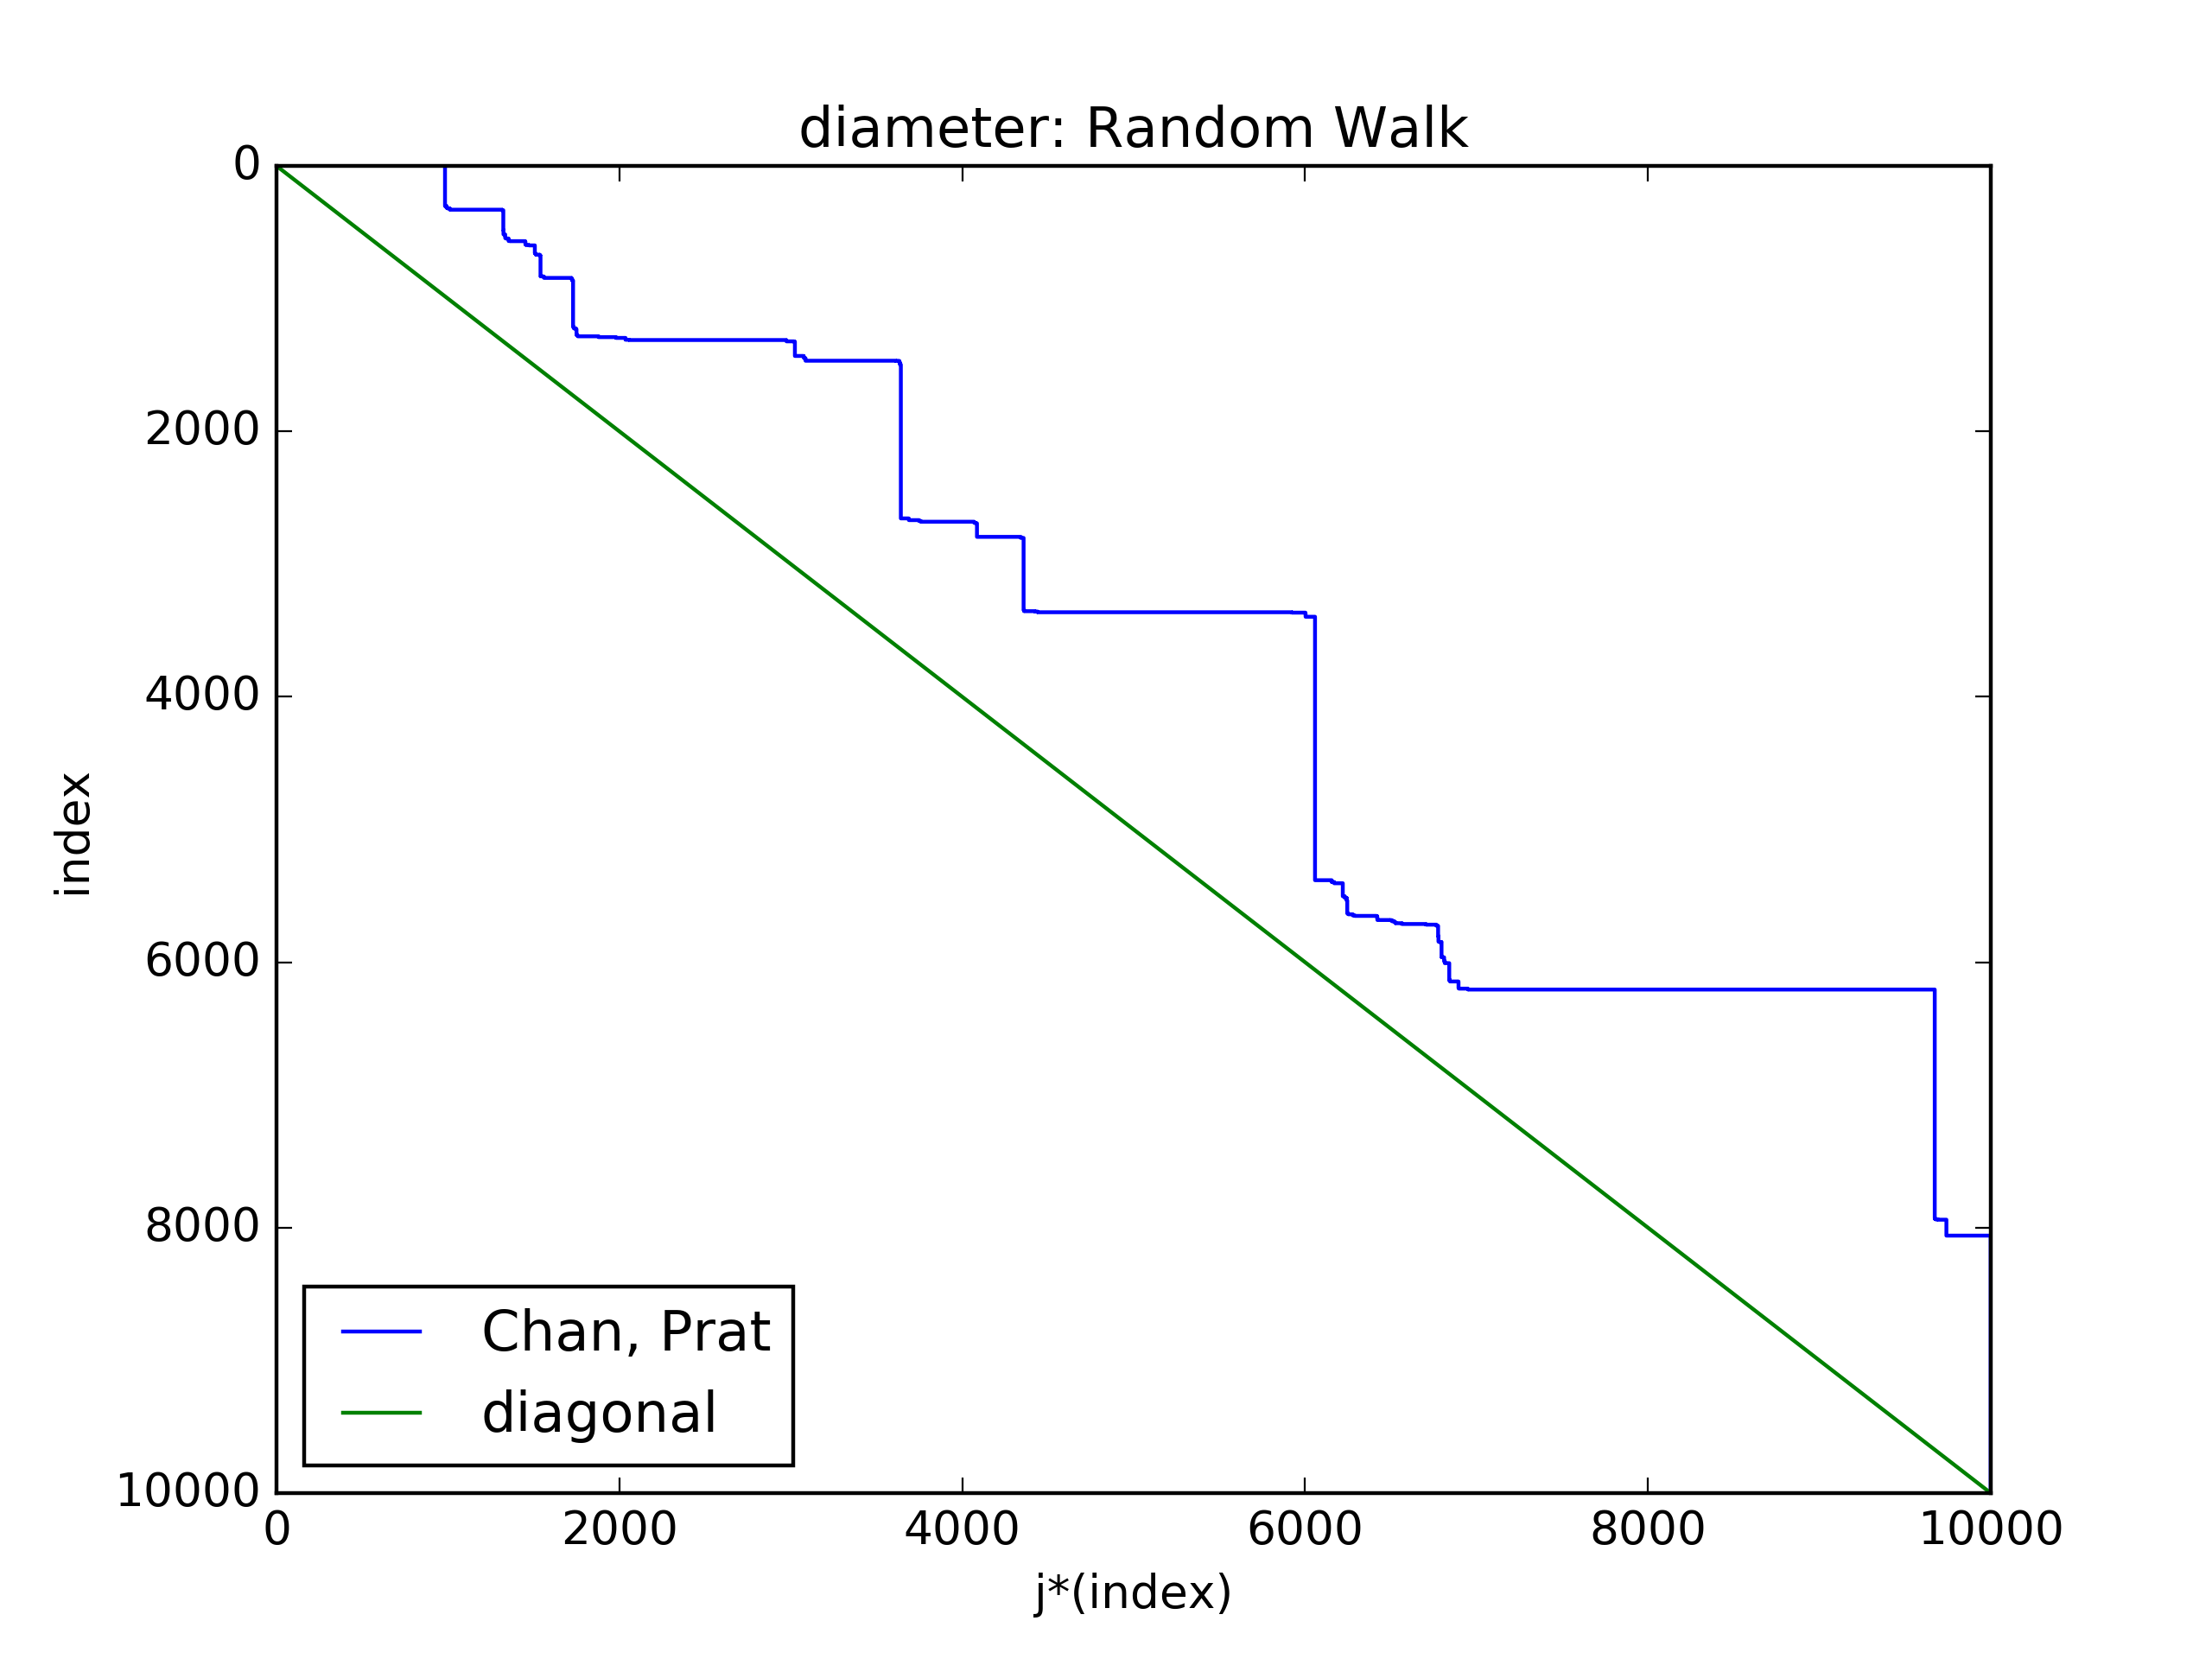
\includegraphics[height=8cm]{plots/diameter_random_walk}
  \caption{Caption...}
  \label{fig:diameter_demo}
\end{figure}

\begin{figure}[!h]
  \centering
  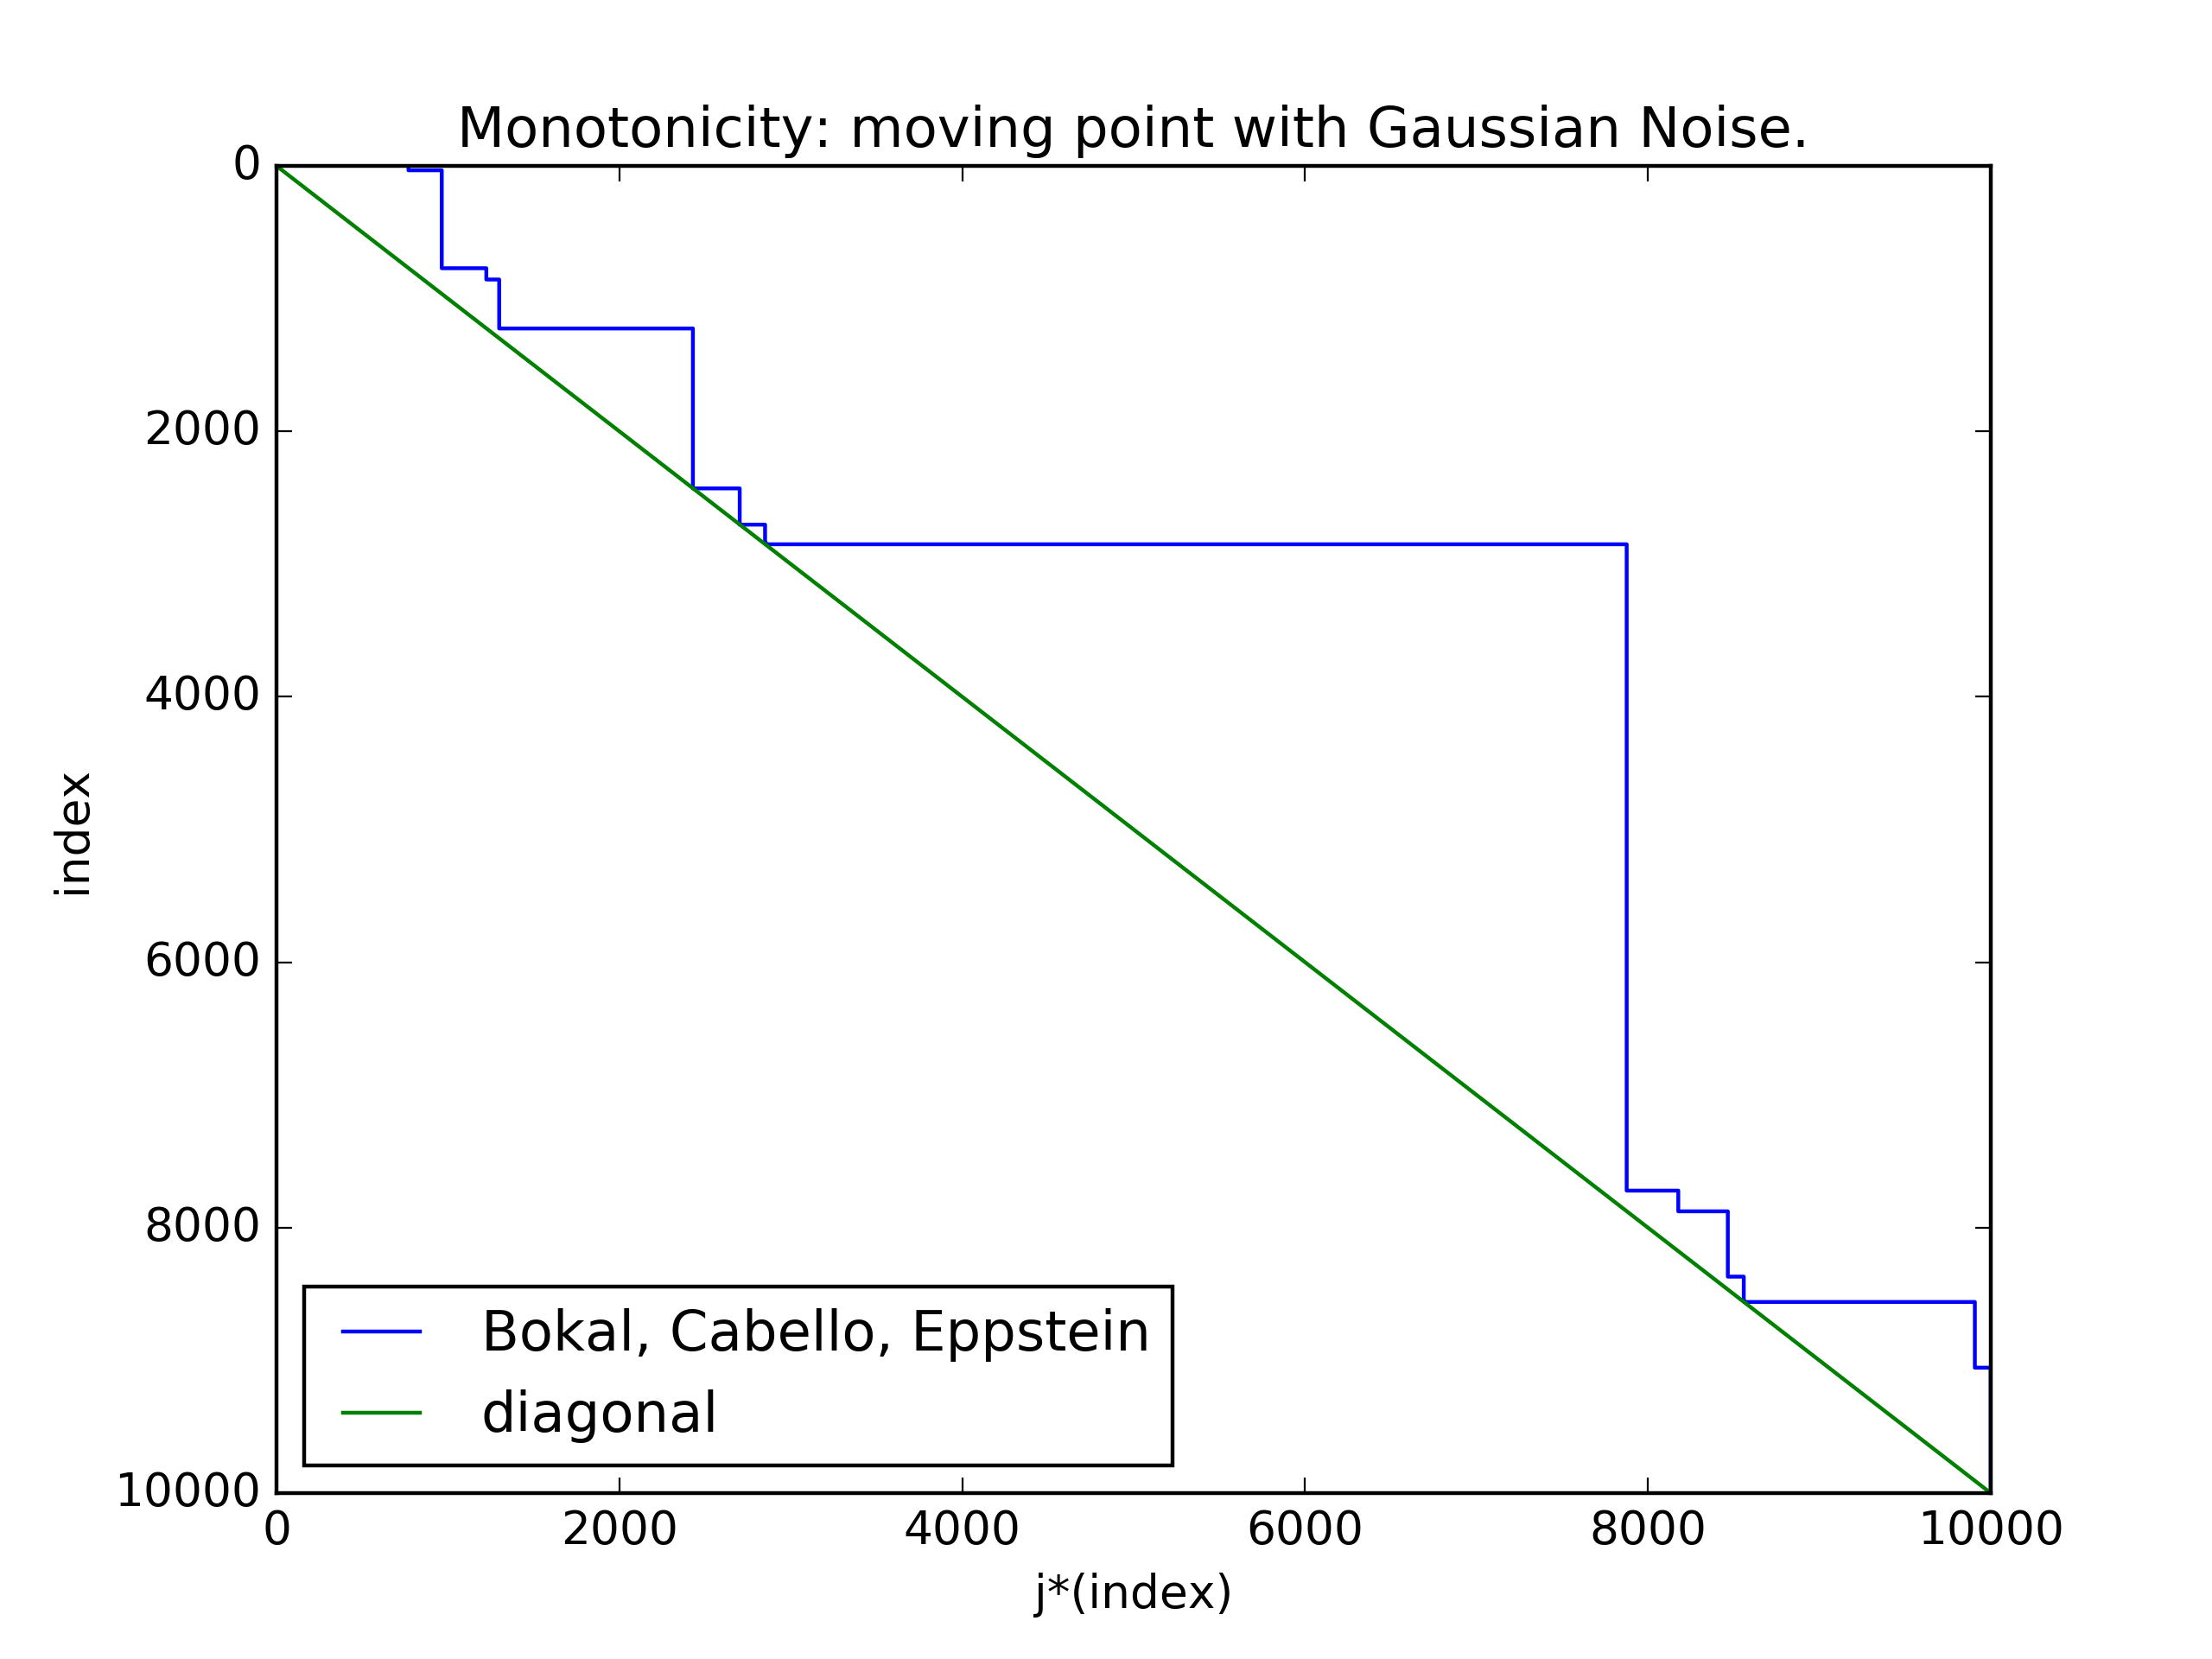
\includegraphics[height=8cm]{plots/monotonicity_moving_gaussian}
  \caption{Caption...}
  \label{fig:monotonicity_demo}
\end{figure}

\section{Conclusion}
This was a great project!

\bibliographystyle{unsrt}
\bibliography{papers}
\end{document}
